%!TEX root = ../thesis.tex
%*******************************************************************************
%****************************** Fifth Chapter **********************************
%*******************************************************************************
\chapter{Ballistic Deposition With Redefinition of Site Percolation}
\label{chapter.redefinition--ballistic-deposition}
% **************************** Define Graphics Path **************************
\ifpdf
    \graphicspath{
    	{Chapter4/Figs/}
    	{Chapter5/Figs/}
    	{Chapter5/Figs/L0/}
    	{Chapter5/Figs/L1/}
    	{Chapter5/Figs/L2/}
    	{Chapter5/Figs/traditional/}
    	{Chapter5/Figs/lattice/}
    }
\else
    \graphicspath{
    	{Chapter4/Figs/}
		{Chapter5/Figs/}
		{Chapter5/Figs/L0/}
		{Chapter5/Figs/L1/}
		{Chapter5/Figs/L2/}
		{Chapter5/Figs/traditional/}
    	{Chapter5/Figs/lattice/}
    }
\fi


Here we first revisit random site and bond percolation in square lattice focusing primarily 
on entropy which quantifies the degree of disorder and order parameter
that measures the extent of order. Note that being two opposite quantities they can neither be
minimum nor be maximum at the same time which is perfectly consistent 
with bond percolation. However, the same is  not true for traditional site
percolation as we find that entropy and order parameter are both zero at occupation 
probability $p=0$ and the way entropy behaves it violates the second law of thermodynamics. To overcome this we redefine the site percolation 
where we occupy sites to connect bonds and we measure cluster size by the number of bonds connected by occupied sites. 
This resolves the problem without affecting any of the existing known results whatsoever.\\


Then we investigate percolation by random sequential ballistic deposition (RSBD) on a square lattice with interaction range upto second nearest neighbors. The critical points $p_c$ and all the necessary critical exponents $\alpha$, $\beta$, $\gamma$, $\nu$ etc. are obtained numerically for  each range of interactions. Like  in its thermal counterpart, we find that the critical exponents of RSBD depend on the range of interactions and for a given range of interaction they obey the Rushbrooke inequality. Besides, we obtain the  fractal dimension $d_f$ that characterizes the spanning cluster at $p_c$ (\ref{subsect:fractal-dim}). Our results suggest that the RSBD for each range of interaction belong to a new universality class which is in sharp contrast to earlier results of the only work that exhist on RSBD.


\section{Redefinition of Site Percolation}
	\label{sect.redefinition-site-percolation}
	we first define the percolation process and to do it
	we first need to choose a skeleton. It can either be an abstract graph which is now
	better known as network or be a spatially embedded lattice
	which are consist of nodes or site and links or bonds.  
	A square lattice of linear size $L$ has 
	$L^2$ sites connected by $2L^2$  bonds with periodic boundary condition and by
	$2L(L-1)$ bonds without periodic boundary condition. Percolation 
	is known as site or bond type depending on whether we occupy sites or bonds respectively.
	In section (\ref{bond-percolation}) we have described the bond percolation and we have seen that we occupy bond to connect clusters of different sizes.

	
	Interestingly, we find that the way the 
	relative size of the spanning cluster $P=s_{{\rm span}}/N$ varies 
	with $p$ such that $P=0$ for $p\geq p_c$ and $P\sim (p-p_c)^\beta$. This is reminiscent of the order parameter of continuous phase transition
	and hence $P$ is regarded as the order parameter for percolation \cite{Stanley1987, Binney1992}.
	This is one of the reasons why scientists in general and physicists in particular find percolation theory so attractive. 
	
	
	
	We still have many unresolved issues in percolation.  For instance, we know that the
	order parameter measures the extent of order but we do not yet 
	know what order really is in percolation. Note that $P=0$
	in the entire disordered phase at least in the thermodynamic limit. We therefore need another
	quantity that can quantify the degree of disorder in the disordered phase. 
	The obvious choice is entropy without which
	any model for phase transition is incomplete since, like order parameter, it is also used to define
	the order of transition. In the case of first order transition, entropy is discontinuous
	at the critical point and the corresponding gap is proportional to the latent heat.
	Despite being such an important quantity, its definition remained elusive in percolation until our 
	recent work in 2017 \cite{Hassan2017, Sabbir2018}.
	Note that both entropy and the order
	parameter cannot be minimally low or maximally high at the same time since no system 
	can be in the ordered and disordered at the same time. Thus, they form such a pair that 
	when one is minimally low the other has to be maximally
	high and vice versa. Moreover, the two quantities together characterize whether the transition 
	is accompanied by symmetry breaking or not. 
	Recall that in the continuous thermal phase transition, such as paramagnetic to 
	ferromagnetic transition, the order parameter is maximum, $m\rightarrow 1$ 
	as temperature $T\rightarrow 0$, where entropy is minimum there. On the other hand, the order parameter 
	is zero or minimum where the entropy is maximally high. Meanwhile at and near the critical 
	point both the quantities undergo an abrupt change. It implies that the paramagnetic
	to ferromagnetic transition is an order-disorder transition which also means that the transition
	is accompanied by symmetry breaking.
	
	
	\subsection{Definition of Entropy and Order Parameter}
	
	The two most important quantities of interests in the theory of phase transition and critical phenomena 
	are the entropy $H$ and the order parameter $P$ since they are the ones
	which define the nature of transition. In the first order or discontinuous phase transition,
	entropy must suffers a jump or discontuinity at the critical point which is 
	why first order transition
	requires latent heat. Similarly, the order parameter too must suffer a jump or discontinuity at
	the critical point and that is the why new and old 
	phase can coexist at the same time in the first order transition. Besides, they are also used as a litmus test to check
	whether the transition is accompanied by symmetry breaking or not. In the case of symmetry breaking,
	the system undergoes a transition from the disordered state, which is characterized by maximally high
	entropy, to the ordered state, which is characterized by maximally high order parameter. 
	Such transition happens with an abrupt or sudden
	change in $P$ and $H$ but without gap or discontinuity at $p_c$. 
	Percolation being a probabilistic model for phase transition, there is
	absolutely no room for considering thermal entropy. To this end, the 
	best candidate is definitely the Shannon entropy  
	\begin{equation}
	\label{eq:shannon_entropy}
	H(t)=-K\sum_i^m \mu_i\log \mu_i,
	\end{equation} 
	where we choose $K=1$ since it merely amounts to a choice of a unit of measure of entropy \cite{Shannon1948}. 
	
	
	%\subsection{Order parameter}
	
	On the other hand, the strength $P(p,L)$ of the spanning cluster for system size $L$
	is define as 
	\begin{equation}
	\label{eq:pp1}
	P={{{\rm Number \ of \ bonds \ in \ the \ spanning \ cluster}}\over{{\rm Total \ 
				number \ of \ bonds }=2L^2}}.
	\end{equation}
	Essentially, it describes the probability that a site 
	picked at random belongs to the spanning cluster at occupation probability $p$ for system size $L$.
	It has been found that in the limit $L\rightarrow \infty$ the probability $P(p,L)=0$ 
	for $p\leq p_c$ and it reaches to its maximum value $P(p,L)=1$ 
	following power-law $P\sim (p-p_c)^\beta$ near but above $p_c$. This is reminiscent 
	of the order parameter in the continuous thermal phase transition like magnetization
	during the ferromagnetic transition.  However, for finite system size $P(p,L)$ may have non-zero
	value at $p<p_c$. However, as we increase the size $L$ of the system it always shows a clear sign
	of becoming zero. There exists yet another definition where 
	we can use the size of the largest cluster instead of the spanning cluster. Note that both the definitions 
	behave in the same fashion and have all the properties of the order parameter. That is,  
	in the limit $L\rightarrow \infty$, 
	$P=0$ for $p\leq p_c$ and it rises from $P=0$ at $p_c$ to $P=1$ continuously and monotonically like $P\sim (p-p_c)^\beta$. 
	Such behavior is reminiscent of order parameter like magnetization $m$ in the ferromagnetic transition and
	hence $P$ is regarded as the order parameter in percolation theory. 
	
	
	\subsection{Problem for entropy with traditional site percolation}
	
	We first measure entropy for random bond percolation
	where initially every site is a cluster of its own size. As 
	we keep occupying or reactivating frozen bonds, clusters are continuously formed and
	their sizes on average are grown. Consider that at an arbitrary step of the process
	there are $m$ distinct, disjoint, and indivisible labelled clusters $i=1,2,...,m$ 
	whose sizes are $s_1,s_2,....,s_m$ respectively. We can therefore define 
	$\mu_i=s_i/\sum_i s_i$ as the corresponding cluster picking probability (CPP),
	that a site picked at random belongs to the cluster $i$, which is naturally normalized  $\sum_j s_j=N$  
	\cite{Hassan2017, Hassan2015}. Thus, at $p=0$ we have 
	$\mu_i=1/N$ for all the sites $i=1,2,...,N=L^2$ which is exactly like the state 
	of the isolated ideal gas where all the allowed microstates are equally likely.
	It is thus expected that entropy is maximum $H=\log N$ at $p=0$ revealing  that we are in a state of 
	maximum uncertainty just like the state of the isolated ideal gas.  
	On the other hand, as we go to the other extreme at $p=1$ we find that all the 
	sites belong to one cluster that makes  $\mu_1=1$. It implies
	that entropy is zero at $p=1$ and hence we are in a state of zero uncertainty just like the perfectly 
	ordered crystal structure. In order to see how entropy interpolates between $p=0$ and $p=1$,
	we use CPP in Eq. (\ref{eq:shannon_entropy}) and the resulting entropy is shown
	in  Fig. (\ref{fig:entropy-order-parameter-bond-traditional-site-a}) as a function of $p$ for different system size. 
	
	\begin{figure}[h]
		\centering
		\captionsetup[subfigure]{width=0.9\textwidth}
		\begin{subfigure}[t]{.45\textwidth}
			\centering
			\includegraphics[width=\linewidth]{{{sq_lattice_bond_percolation__periodic___entropy}}}
			\caption{}
			\label{fig:entropy-order-parameter-bond-traditional-site-a}		
		\end{subfigure}
		\begin{subfigure}[t]{.45\textwidth}
			\centering
			\includegraphics[width=\linewidth]{{{sq_lattice_site_percolation_periodic__entropy_by_site-entropy-order_parameter-traditional2-L400}}}
			\caption{}
			\label{fig:entropy-order-parameter-bond-traditional-site-b}	
		\end{subfigure}
		\caption{(a) Entropy $H$ versus $t$ for bond percolation. (b) Entropy (blue) and order parameter (orange) for traditional site percolation. we plot entropy $H(p)/H(0)$ and order parameter $P(p)/P(1)$			in the same graph to see the contrast.}
		\label{fig:entropy-order-parameter-bond-traditional-site}
	\end{figure}
	
	
	
	
	
	To see how entropy for random site percolation 
	differs from that of the bond type we now measure entropy for traditional definition of site percolation. In this case,
	it is assumed that initially all the sites are frozen or empty.
	The process starts with occupation of sites one by one at random and measure
	the cluster size exactly like in the bond percolation.
	It means initially CPP does not exist and after the occupation of the first site $\mu=1$ 
	and hence entropy $H=0$ at $p=1/N$ which is essentially zero
	in the limit $N\rightarrow \infty$.
	As we further occupy sites, we observe a sharp rise in the entropy to its maximum value, 
	see Fig. (\ref{fig:entropy-order-parameter-bond-traditional-site-b}), which happens near $p=0.2$. Thereafter it decreases 
	with $p$ qualitatively in the same way as in the case of random bond type percolation. To see the
	contrast we also show the order parameter also in Fig. (\ref{fig:entropy-order-parameter-bond-traditional-site-b}). This figure
	suggest that at $p\sim 0$ entropy and order parameter  both 
	are zero which cannot be true. Besides, entropy of site percolation violates
	the second law of thermodynamics as it states that entropy of isolated system cannot first
	increase and then decrease again. It thus warrants redefinition of site percolation. 
	
	

	
	
	
	\subsection{Site percolation re-defined}
	
	The questions is: How can we resolve the problem with the definition of traditional site percolation?
	We can get the definition of site percolation
	from the definition of bond percolation simply by replacing bonds with site and vice versa.
	That is, we assume that initially isolated bonds are already
	there in the system which are shown in Fig. (\ref{fig:site-redifined}) by the thick black lines and sites
	are empty (white corcles). We then keep picking one site at each step with uniform probability
	and occupy it to connect four bonds around it.  
	
	 
	\begin{figure}[h]
		\centering
		\captionsetup[subfigure]{width=0.9\textwidth}
		\begin{subfigure}[t]{.45\textwidth}
			\centering
			\includegraphics[width=5cm]{{{site-square-lattice-5x5_def}}}
			\caption{}
			\label{fig:site-redifined-a}
		\end{subfigure}
		\begin{subfigure}[t]{.45\textwidth}
			\centering
			\includegraphics[width=5cm]{{{site-square-lattice-5x5_cluster-1}}}
			\caption{}
			\label{fig:site-redifined-b}
		\end{subfigure}
		\caption{(a) Illustration of redefined site percolation on square lattice. We assume that process			starts with isolated bonds (thick black 			lines)  but sites are empty (white circles). (b) Occupying one site connects four bonds hence it forms a cluster of size four.} 
		\label{fig:site-redifined}
	\end{figure}

	We measure cluster size by the number of bonds that it contains and occupation probability as the fraction of the sites
	being occupied. For instance, the cluster of size four is shown in Fig. (\ref{fig:site-redifined-b}) by green color.
	Using this renewed definition, we again measure entropy and find entropy is just like
	its bond counterpart. That is, entropy is 
	maximum at $p=0$ and  as $p$ approaches $p_c$ it drops sharply. It then again decreases slowly
	to zero as $p$ reaches its maximum value $p=1$ which is shown in Fig. (\ref{fig:site-redifined-entropy-order-parameter-a}). We
	clearly see that its qualitative behaviour is exactly the same as   Fig. (\ref{fig:entropy-order-parameter-bond-traditional-site-a}) for the bond 
	percolation and hence the problem of absurdity, that entropy and order parameter both
	equal to zero at $p=0$, and the violation of the second law of thermodynamics are resolved.
	
	\begin{figure}[h]
		\centering
		\captionsetup[subfigure]{width=0.9\textwidth}
		\begin{subfigure}[t]{.45\textwidth}
			\centering
			\includegraphics[width=7cm]{{{sq_lattice_site_percolation_periodic_-entropy}}}
			\caption{}
			\label{fig:site-redifined-entropy-order-parameter-a}
		\end{subfigure}
		\begin{subfigure}[t]{.45\textwidth}
			\centering
			\includegraphics[width=7cm]{{{sq_lattice_site_percolation_periodic__entropy_by_site-entropy-order_parameter-L400}}}
			\caption{}
			\label{fig:site-redifined-entropy-order-parameter-b}
		\end{subfigure}
		\caption{For redefined site percolation we plot (a) Entropy. (b) Entropy $H(t)/H(0)$ and order parameter $P(t)/P(1)$	in the same graph to see the contrast.  It can be easily seen that $P=0$ where			entropy is maximally high and order parameter is maximally high where entropy is minimally low			which is reminiscent of order-disorder transition in the ferromagnetic transition.
		}
		\label{fig:site-redifined-entropy-order-parameter}
	\end{figure}

	
	
	Perhaps plots of entropy and order parameter
	in the same graph can help us appreciate their opposing nature better than they are shown separately. 
	Note that the numerical value of the maximum 
	entropy, which is equal to $\log (N)$, is much higher than the maximum value of $P$ which is equal to one. 
	We, therefore, measure relative entropy $H(p)/H(0)$ and relative order parameter $P(p)/P(1)$ 
	in an attempt to re-scale their values so that in either cases their respective maximum values become
	unity. The plots of re-scaled entropy and order parameter
	are shown in Fig. (\ref{fig:site-redifined-entropy-order-parameter-b}) which clearly shows that $H$ is maximally high where $P=0$ and the order parameter is maximally high 
	where $H$ is minimally low. Besides, they both undergo a sharp change in the vicinity of the critical point $p_c$ and consistent with the second law of thermodynamics. This is exactly what is expected as order
	parameter measures the extent of order and entropy quantifies the degree of disorder. 
	It means that percolation transition 
	is accompanied by symmetry breaking just like paramagnetic to ferromagnetic
	transition. In other words 
	it is an order-disorder transition since in one phase $P=0$ and $H$ is maximally high revealing
	it corresponds to disordered phase and in the other phase $P$ is maximally height but $H$ is minimally low revealing
	it is the ordered phase.
	
	
	
	

	
	
	
	\subsection{Is site-bond universality still valid?}
	
	
	We now check if the re-defined site percolation still gives the
	same critical point $p_c=0.5927$ and the same the critical exponent $\nu$ of the equivalent
	counterpart of the coorelation length or not.
	The best quantity for finding the critical point $p_c$ and critical exponent $\nu$ is the
	spanning probability $W(p)$. It describes the likelihood of finding a 
	cluster that spans across the entire system
	either horizontally or vertically at a given occupation probability $p$.
	In Fig. (\ref{fig:site-redefine-spanning-probability-a}) we show $W(p)$ as a function of suitable class of width $\Delta p$
	which is essentially the plot os $W(p)$ as a function of
	$p$ for different system sizes $L$. One of the significant features of such plots is that they all 
	meet at one particular value regardless of the value of $L$. It 
	is actually the critical point $p_c=0.5927$
	which is exactly the same known value as for the traditional definition of site percolation. 
	
	
	\begin{figure}[h]
		\centering
		\captionsetup[subfigure]{width=0.9\textwidth}
		\begin{subfigure}[t]{0.4\textwidth}
			\centering
			\includegraphics[width=\linewidth]{{{sq_lattice_site_percolation_periodic_-occupation_probability-pc0.5927}}}
			\caption{}
			\label{fig:site-redefine-spanning-probability-a}
		\end{subfigure}
		\begin{subfigure}[t]{0.4\textwidth}
			\centering
			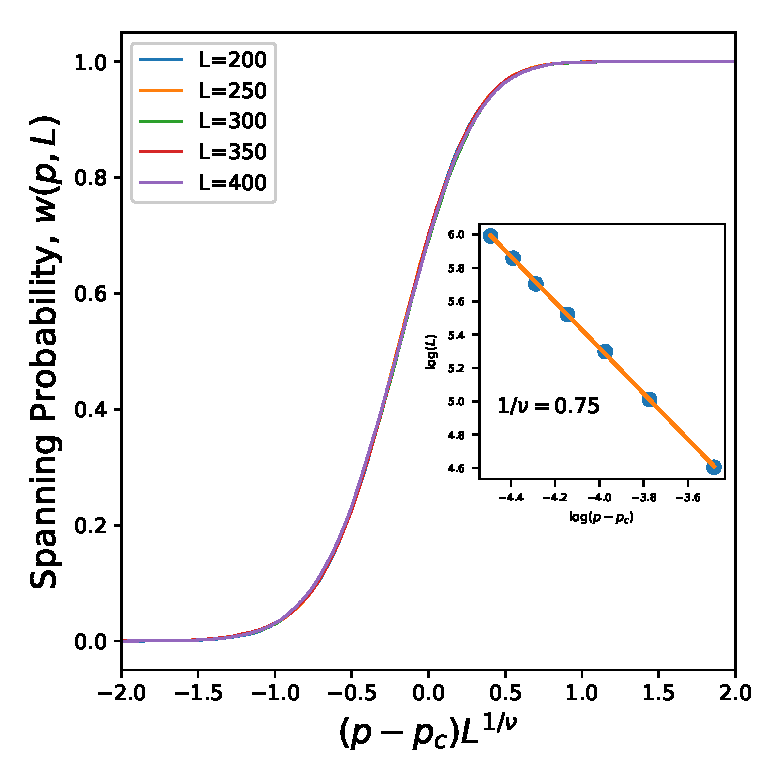
\includegraphics[width=\linewidth]{{{L0/sq_lattice_site_percolation_periodic_-occupation_probability-data_collapse-pc0.5927-ex0.7500}}}
			\caption{}
			\label{fig:site-redefine-spanning-probability-b}
		\end{subfigure}
		\caption{(a) Spanning probability $W(p,L)$ vs $p$ for different lattice sizes using new definition
			of site percolation. 
			In (b) we plot dimensionless quantities $W$ vs $(p-p_c)L^{1/\nu}$ using known value of $\nu=4/3$
			and find excellent data-collapse which is a proof that bond-site still belong to the same universality class.
		} 
		\label{fig:site-redefine-spanning-probability}
	\end{figure}
	
	
	Thus, the value of $p_c$ does not depend on whether we measure the cluster size
	in terms of the number of sites or the number of bond it contains.
	Note that finding the $p_c$ value for different skeletons
	is one of the central problems in percolation theory \cite{Ziff2009, Ziff2010}. 
	To check whether the $\nu$ value is still the same we use its standard known value
	$\nu=4/3$ \cite{Ziff1992}. We then plot of $W(p)$ vs $(p_c- p)L^{{{1}\over{\nu}}}$ and
	find that all the distinct curves of Fig. (\ref{fig:site-redefine-spanning-probability-a}) collapse into a universal 
	scaling curve as shown in Fig. (\ref{fig:site-redefine-spanning-probability-b}) for $\nu=4/3$. This is a clear testament
	that the critical point $\nu$ is also the same as that of the traditional site percolation.  
	
	


	Next we attempt to find the critical exponent $\beta$ of the order parameter $P$ using 
	the new definition of site percolation.
	First we plot order parameter $P(p)$ in Fig. (\ref{fig:site-redefine-order-parameter-a})  as a function of $p$ for different
	lattice size $L$. We now use the
	standard known values for $\nu=4/3$ and $\beta/\nu=0.104$ and plot  $P(p,L)L^{\beta/\nu}$ versus
	$(p-p_c)L^{1/\nu}$ in Fig. (\ref{fig:site-redefine-order-parameter-b}). We get an excellent data collapse revealing that the new definition of site
	percolation reproduces the known value of $\beta=0.1388$ in $2d$ random percolation. 
	It confirms that the site-bond universality
	is not affected by the new definition. Recently, we have also studied random percolation 
	on scale-free lattice and found that $\beta=0.222$ 
	\cite{Hassan2015}. 
	This is the only exception that, despite the dimension of the embedding space of the scale-free weighted planar stochastic lattice is two, yet it belongs to different universality class. 
	
	\begin{figure}[h]
		\centering
		\captionsetup[subfigure]{width=0.9\textwidth}
		\begin{subfigure}[t]{0.4\textwidth}
			\centering
			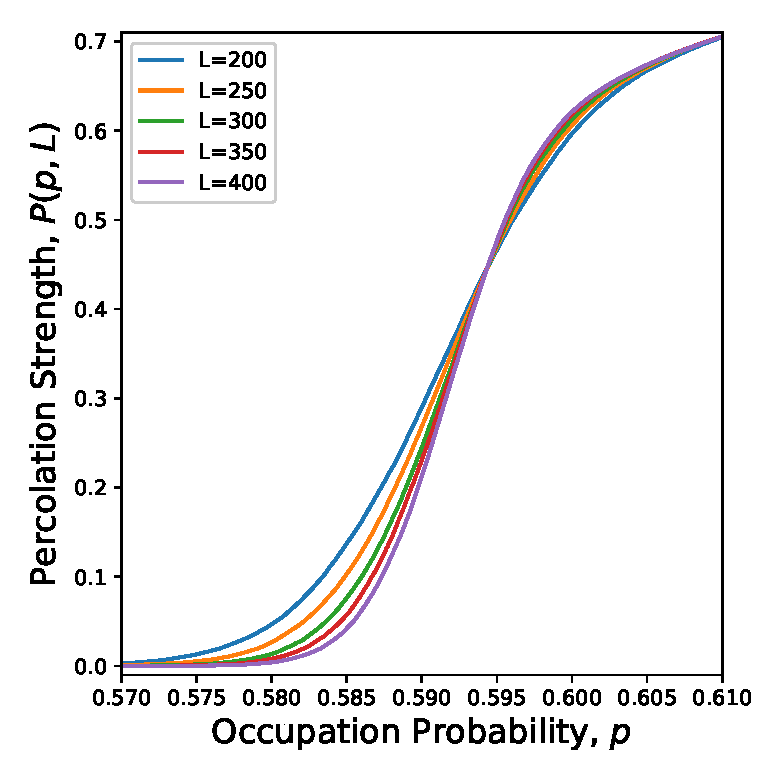
\includegraphics[width=\linewidth]{{{L0/sq_lattice_site_percolation_periodic_-spanning-_order_parameter-pc0.5927}}}
			\caption{}
			\label{fig:site-redefine-order-parameter-a}
		\end{subfigure}
		\begin{subfigure}[t]{0.4\textwidth}
			\centering
			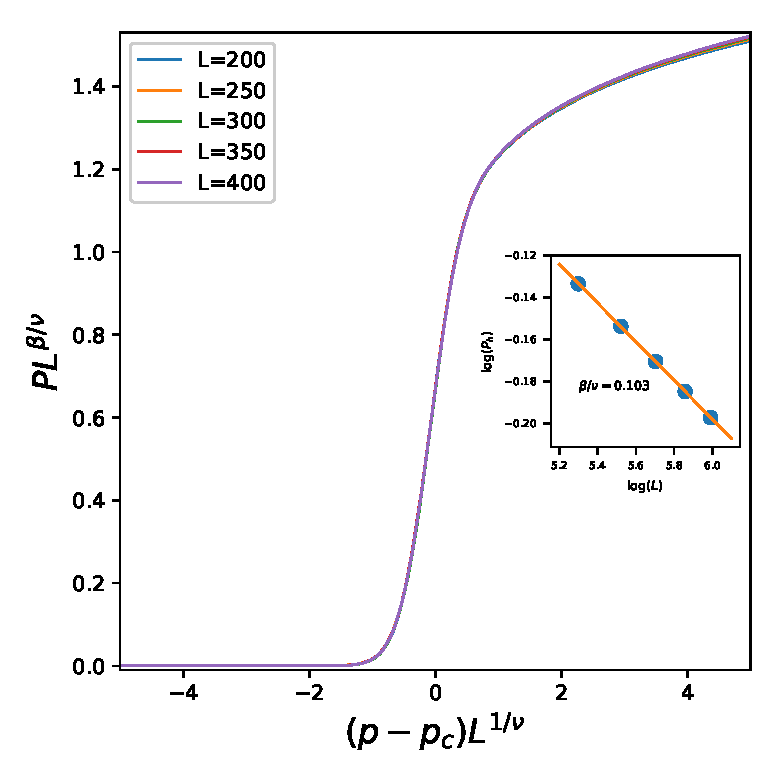
\includegraphics[width=\linewidth]{{{L0/sq_lattice_site_percolation_periodic_-spanning-_order_parameter-data_collapse-pc0.5927_beta_0.103_nu_0.750}}}
			\caption{}
			\label{fig:site-redefine-order-parameter-b}
		\end{subfigure}
		\caption{(a) Order parameter $P(p,L)$ vs $p$ for re-defined site percolation in the square lattice. 
			(b) We plot $P(p,L)L^{\beta/\nu}$ versus $(p-p_c)L^{1/\nu}$ using know value of $\nu=4/3$ and $\beta=5/36$. 
			An excellent data collapse proves that our way defining site percolation can still reproduce the
			same critical exponents. 
		}
		\label{fig:4ab}
		\label{fig:site-redefine-order-parameter}
	\end{figure}
	
	
	Knowing the entropy pave the way of obtaining the
	specific heat since we know that it is proportional to the first derivative of entropy
	i.e. $C=TdS/dT$ where $S$ is the thermal entropy. If we now know the exact equivalent 
	counterpart of temperature
	then we can immediately obtain the specific heat for percolation. In our recent work we
	argued that $1-p$ is the equivalent counterpart of temperature and hence the specific
	heat for percolation is 
	\begin{equation}
	C(p)=(1-p){{dH}\over{d(1-p)}}.
	\end{equation}
	The plots of $C(p)$ as a function of $p$ for different
	system size $L$ is shown in Fig. (\ref{fig:site-redefine-specific-heat-a}). 
	We already know the value of $\alpha=0.906$ from our recent work on bond percolation in
	the square lattice \cite{Hassan2017}. Using the the same values for $\alpha$ and $\nu$
	we plot $CL^{-\alpha/\nu}$ vs $(p-p_c)L^{1/\nu}$ in Fig. (\ref{fig:site-redefine-specific-heat-b}) and find an excellent 
	data collapse. It confirms that $\alpha= 0.906$ is indeed the
	same for both bond and redefined site percolation.
	
	\begin{figure}[h]
		\centering
		\captionsetup[subfigure]{width=0.9\textwidth}
		\begin{subfigure}[t]{0.4\textwidth}
			\centering
			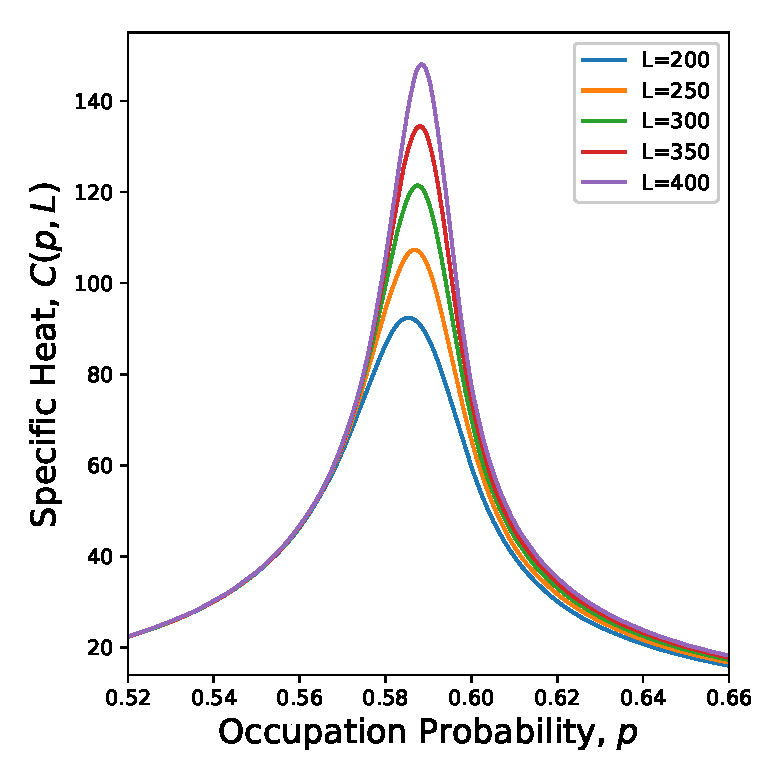
\includegraphics[width=\linewidth]{{{L0/sq_lattice_site_percolation_periodic__specific_heat-pc0.5927}}}
			\caption{}
			\label{fig:site-redefine-specific-heat-a}
		\end{subfigure}
		\begin{subfigure}[t]{0.4\textwidth}
			\centering
			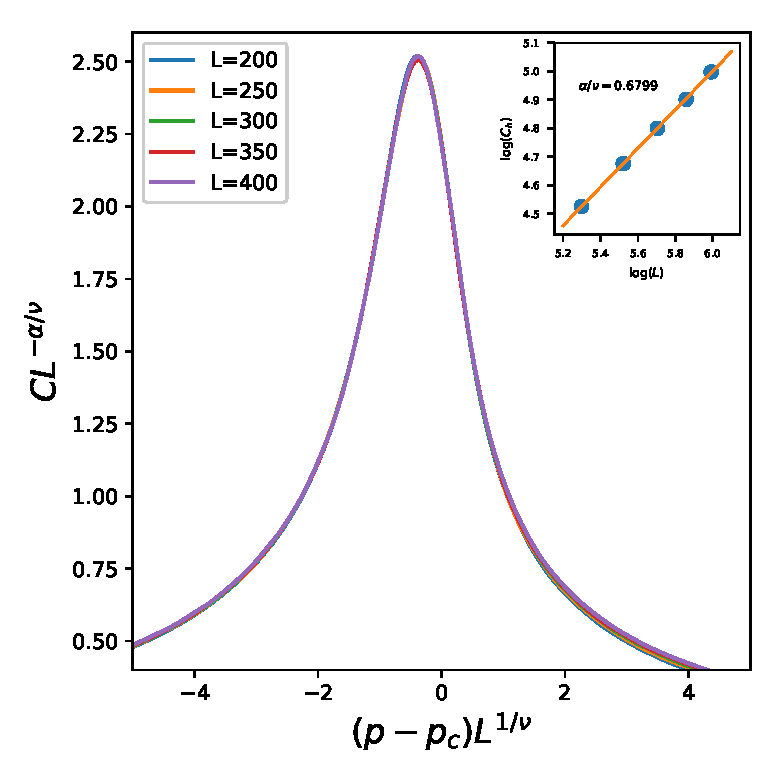
\includegraphics[width=\linewidth]{{{L0/sq_lattice_site_percolation_periodic__specific_heat-data_collapse-pc0.5927_alpha_0.6799_nu_0.750}}}
			\caption{}
			\label{fig:site-redefine-specific-heat-b}
		\end{subfigure}
		\caption{Specific heat $C(p,L)$ vs $p$ in square lattice for re-defined site percolation. 
			In (b) we plot dimensionless quantities $CL^{-\alpha/\nu}$ vs $(p-p_c)L^{1/\nu}$ and we find an excellent data-collapse.
		} 
		\label{fig:site-redefine-specific-heat}
	\end{figure}
	
	
	
	
	In percolation, yet another quantity of interest is the susceptibility. 
	Traditionally, mean cluster size
	has been regarded as the equivalent counterpart of susceptibility. Sometimes variance of the order parameter $\sqrt{\langle P^2\rangle -\langle P\rangle^2}$ too is
	regarded as susceptibility. Neither of the two actually gives respectable value for $\gamma$ to obey the
	Rusbrooke inequality. Recently, we proposed susceptibility $\chi(p,L)$ for percolation as
	the ratio of the change
	in the order parameter $\Delta P$  and the magnitude of the time interval $\Delta t$ during which 
	the change $\Delta P$  occurs.  Essentially it becomes the derivative of the order parameter $P$ since
	$\Delta p\rightarrow 0$ in the limit  $N\rightarrow \infty$ as $\Delta p={{1}\over{2L^2}}$. The idea
	of jump has been studied first by Manna in the context of explosive percolation \cite{Manna2012}.
	The resulting susceptibility is shown
	in Fig. (\ref{fig:site-redefine-susceptibility}) as a function of $p$. We already know that $\gamma/\nu=0.6407$ for 
	bond percolation in the square lattice. Using the same value for redefined
	site percolation in the plot of $\chi L^{-\gamma/\nu}$ vs $(p-p_c)L^{1/\nu}$ 
	we find that all the distinct curves in Fig. (\ref{fig:site-redefine-susceptibility-a}) collapse superbly to give Fig. (\ref{fig:site-redefine-susceptibility-b}). It implies
	once again that bond and redefined site percolation share the same $\gamma$ value.
	
	\begin{figure}[h]
		\centering
		\captionsetup[subfigure]{width=0.9\textwidth}
		\begin{subfigure}[t]{0.4\textwidth}
			\centering
			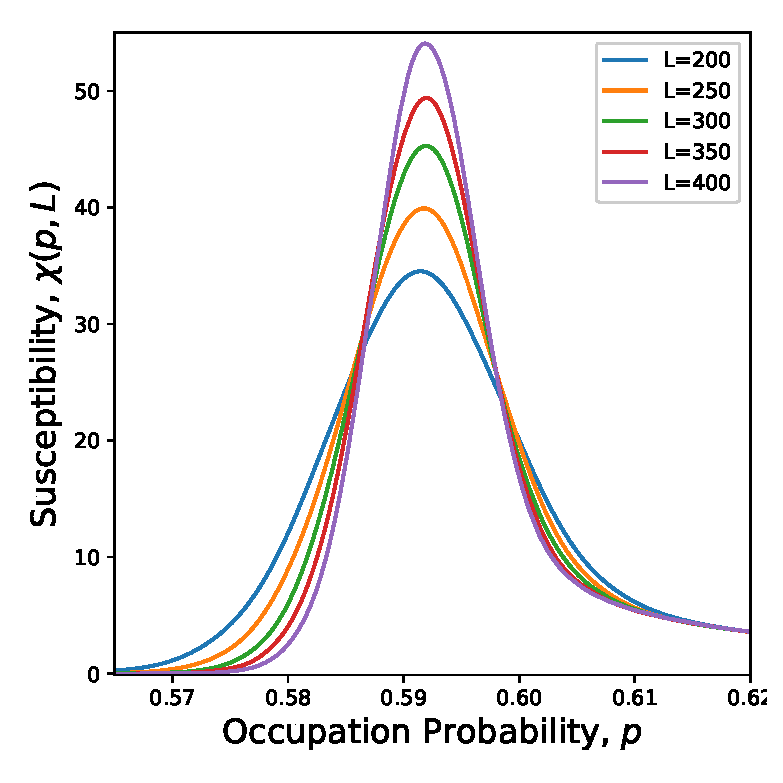
\includegraphics[width=\linewidth]{{{L0/sq_lattice_site_percolation_periodic__susceptibility-pc0.5927}}}
			\caption{}
			\label{fig:site-redefine-susceptibility-a}
		\end{subfigure}
		\begin{subfigure}[t]{0.4\textwidth}
			\centering
			\includegraphics[width=\linewidth]{{{sq_lattice_site_percolation_periodic__susceptibility-data_collapse-pc0.5927_gamma_0.6407_nu_0.750}}}
			\caption{}
			\label{fig:site-redefine-susceptibility-b}
		\end{subfigure}
		\caption{(a) Plots of susceptibility $\chi(p)$ for redefined site percolation as a
			function of $p$ in square lattice of different sizes. 
			In (b) we plot dimensionless quantities $\chi L^{-\gamma/\nu}$ vs $(p-p_c)L^{1/\nu}$ and we find an excellent data-collapse with $\gamma=0.853$ which is the same as for bond type.
		} 
		
		\label{fig:6ab}
		\label{fig:site-redefine-susceptibility}
	\end{figure}
	
	
	\subsection{Fractal Dimension}
	At critical point the square lattice shows the property of a fractal \cite{Falconer2003} (\ref{subsect:fractal-dim}). We use the relation
	\begin{equation}
	S \sim L^{d_f}
	\label{eqn:fractal-dim-1}
	\end{equation}
	taking $\log$ we get
	\begin{equation}
	\log(S) = d_f \log(L)
	\end{equation}
	Here $S$ is the average size of the spanning cluster at critical point. Using this we get the figure (\ref{fig:fractal-dimension}). And we obtain fractal dimension $d_f$ for $L0$ which is listed in (\ref{tab:exponents}). 

	Fractal dimension gives us the information about the size of the spanning(wrapping) cluster. If the lattice size is known we can estimate the average size of the spanning cluster using $d_f$ and (\ref{eqn:fractal-dim-1}).
	
	\begin{figure}
		\centering
		\includegraphics[width=7cm]{{{sq_lattice_site_percolation_periodic_-fractal_dimension_1.89394}}}
		\caption{We plot $\log(S)$ vs $\log(L)$ where $S$ is the size of the spanning cluster and $L$ is the length of the lattice. We obtain the slope $1.8939$  which is the fractal dimensions of the system at $p_c$.}
	\end{figure}

		
		



\section{Random Sequential Ballistic Deposition}
	Imagine a spherical shaped object, say marble, is thrown on top of a 2D square lattice structure. First possible scenario is that the marble will be deposited in the first encountered site in the lattice . Now if the first encountered site is not empty, the possible scenario is that the marble will go in any of the four direction, $+x$, $-x$, $+y$ or $-y$, assuming no other direction in between is allowed in the lattice.  Now if the first neighbor is not empty then the marble will continue to go on in the previously selected direction and choose the next neighbor. This is another topic of this thesis. Others have done some work in this topic \cite{Choi1995, Talbot1992, Jullien1992, Viot1993}. And we have found that for a different range of interaction model they all belong to different universality classes.
	
	
	In our experiment, we occupy a randomly chosen site if it is empty else we select one of its four neighbor to occupy if it is empty else select next neighbor in that direction and occupy that site if it is empty else ignore current iteration and choose another site randomly. This process is repeated until there is no empty site in the lattice. We call this process the ballistic deposition on the square lattice. We introduce 1st and 2nd nearest neighbor interaction in this way.

	Random percolation (RP) model can also be seen as a random sequential adsorption (RSA) \cite{Jullien1992} process of particles on a given substrate to form monolayers of clusters of complex shape and structures. In RSA, a site is first picked at random and it is occupied if it is empty and the trial attempt is rejected if it is already occupied. We shall first show that this process too reproduce all the existing results of the CRP including the $p_c$ value. We can modify the rejection criterion. First, we assume that the adsorbing particles are hard sphere and impenetrable. Then we assume that if a particle fall onto an already adsorbed particle it is not straightaway rejected. Instead, it is allowed to roll down over the already deposited particle to one of its nearest neighbours at random following the steepest descent path. The particle is then adsorbed permanently if the nearest neighbour is empty else the trial attempt is rejected. This is known as the ballistic deposition (BD) \cite{Choi1995, Talbot1992, Jullien1992, Viot1993} model for $l = 1$. We also consider the case that if the nearest neighbour is occupied then the incoming particle attempt to push the neighbour to its next neighour site along the same line to make room for itself. However, the trial attempt of pushing the neighbour is successful if the next neibhouring site along the same line is empty else the trial attempt is discarded. We regard it as BD model for $l = 2$ while the classical percolation correspond to BD model with $l = 0$. Our primary goal is to prove that the critical exponents of percolation changes as changes as we increase the range of interaction like we find in its thermal counterpart. We numerically find the various necessary critical exponents and find that BD for each different range of interaction belong to different universality class and each universality class obeys the Rusbrooke inequality.
	
	Percolation is all about configuration of clusters of deposited particles and the investigation of the emergence of a large-scale connected path created by clusters formed by contiguous diposited particles. We use extensive Monte Carlo simulation on a square lattice with the usual periodic boundary condition to study site percolation according to RSBD rule.\\
	
	The algorithm of the percolation by RSBD can be described as follows. We first label all the sites
	row by row from left to right starting from the top left corner. That is, we first label the first row from
	left to right as $i=1,2,...,L$, the second row again from left to right as $i=L+1,L+2,....,2L$
	and we continue this till we reach the bottom row which we label as $i=(L-1)L+1,...,L^2$. 
	Then at each step we pick a discrete random number $R$ from $1,2,...,L^2-1,L^2$ using uniform random number
	generator and check if the site it represents is already occupied or not. If it is
	empty we occupy it straightaway and move on to the next step. Else we pick one of its neighbours at random. 
	The second attempt in the same step, that mimic the roll over mechanism, is successful if the neighbour
	it picks is empty and if not the trial attempt to deposit is rejected permanently and we move on to the next 
	step anyway. This process is
	repeated over and over again till we want it to stop. We call it RSBD of degree one. We also consider
	the case of RSBS of degree two where the trial attempt is made to occupy the second nearest neighbour too.
	In this case if the incoming particle that fall onto an already occupied site and find its 
	neighbour is ocupied too but the next nearest neighbour site is empty then the neighbour move to the empty
	site to make space for the incoming particle to be deposited there. 
	
	In the following sections we study the threshold for $L1$ and $L2$. Then we find out the critical exponents $\alpha, \beta, \gamma, \nu$ for $L1$ and $L2$. We find that they all satisfy the Rushbrooke inequality which is listed in section (\ref{chapter.summary}). Then we find the fractal dimension of the system at threshold.


	\label{sect:finding-numerical-values}
	\subsection{Critical occupation probability, $p_c$} 
	\label{subsect:finding-pc}
	When we occupy sites of the square lattice, initially, there are only clusters of size $1$. As we keep occupying different size of clusters starts to appear. At a certain point a special cluster appears which spans the entire lattice. We call this cluster the \textit{Spanning Cluster}. It should be noted that the spanning cluster is a special property of the lattice and the appearance of the spanning cluster is considered the phase transition. At the point where the spanning cluster first appears is called the critical point and denoted by $p_c$, meaning the occupation probability at the critical point. The figure (\ref{fig:spanning-probability}) shows the graph of the spanning probability, $W(p,L)$, versus the occupation probability $p$ for different interactions ($L1, L2$) for different lengths. We have found that $p_c$ is $0.5782, 0.5701$ for $L1, L2$ respectively. From figure (\ref{fig:site-redefine-spanning-probability-a}) we know the $p_c$ value for $L0$ and it is $0.5927$. Thus for long range interaction $p_c$ is smaller than for short range interaction. 
		\begin{figure}[h]
			\centering
			\captionsetup[subfigure]{width=0.9\textwidth}
			\begin{subfigure}{0.4\textwidth}
				\centering
				\includegraphics[width=\linewidth]{{{sq_lattice_site_percolation_ballistic_deposition_L1_periodic_-occupation_probability-pc0.5782}}}
				\caption{}
			\end{subfigure}
			\begin{subfigure}{0.4\textwidth}
				\centering
				\includegraphics[width=\linewidth]{{{sq_lattice_site_percolation_ballistic_deposition_L2_periodic_-occupation_probability-pc0.5701}}}
			\caption{}
			\end{subfigure}
			\caption{Spanning probability $W(p,L)$ vs $p$ for different lattice sizes using new definition
				of site percolation for (a) $L1$ and (b) $L2$ interaction. We find the threshold (critical point) which is the intersection of curves of different lattice sizes and we get $0.5782$ and $0.5701$ as $p_c$ for (a) $L1$ and (b) $L2$. 
			}
			\label{fig:spanning-probability}
		\end{figure}
	The quantity $w(p, L)$ is called the spanning probability in a non periodic case and wrapping probability in a periodic case.
	The question is how do we find the wrapping probability, given that we have a list of $p_c$ for different length. Note that for a certain length $L$, in each realization the $p_c$ is not exact value, instead it is a range of values that contains the $p_c$. For example, say we have a lattice of length $200$ and for that we will have different $p_c$ at each realization. After an infinite number of experimentation we will have to take an average and that will give the exact value of $p_c$. But since it is practically impossible, we can find $p_{c_{avg}}$ for different lattice size then from the graph we can extrapolate the exact value of $p_c$ for infinite lattice. Here $p_{c_{avg}}$ is calculated from a finite set of $p_c$ for a certain length. This process is not good enough. Since it requires  $p_{c_{avg}}$'s for a number of lattice size which is very costly to obtain. But from the data, list of $p_c$'s for different length, we can find the cumulative frequency distribution. It is astonishing  that for all length the wrapping probability coincide at a specific point. This implies that if we could have an infinite system, the wrapping probability for that system would have gone through this same point. This means we have got our critical point, $p_c$, as the intersection of the $W(p,L)$ for different lengths.
	
	\clearpage
	\newpage
	\subsection{Spanning Probability and finding $1/\nu$} \label{subsect:spanning-probability-and-one-by-nu}
	From the figure (\ref{fig:spanning-probability}) we can see that, as we increase the length of the lattice the wrapping probability $W(p,L)$ moves closer and closer to the critical point. And if we draw a horizontal line at a certain height (close to the bottom), say $y=0.15$, and find the intersection of this line with $W(p,L)$ for each length  and note the $p$ and if we plot $\log(L)$ vs $\log(p-p_c)$ we get the slope $1/\nu$. which is shown in the inset of the figure (\ref{spanning-probability-data-collapse}).
	\begin{figure}[h]
		\centering
		\captionsetup[subfigure]{width=0.9\textwidth}
		\begin{subfigure}[t]{0.4\textwidth}
			\centering
			\includegraphics[width=\linewidth]{{{sq_lattice_site_percolation_ballistic_deposition_L1_periodic_-occupation_probability-hline-pc0.5782}}}
			\caption{}
		\end{subfigure}
		\begin{subfigure}[t]{0.4\textwidth}
			\centering
			\includegraphics[width=\linewidth]{{{sq_lattice_site_percolation_ballistic_deposition_L2_periodic_-occupation_probability-hline-pc0.5701}}}
			\caption{}
		\end{subfigure}
		\caption{A horizontal line is plotted at height $h\sim 1.5$ which at the bottom of the graph. We measure the distance from the vertical line (black) to the intersection of the curves for different lattice size, $L$ and call them $(p-p_c)$ where $p_c$ is the critical point (black line). The plot of $\log(L)$ vs $\log(p-p_c)$ gives us the exponent that scales the $x$-values of this curves.}
		\label{fig:spanning-probability-with-hline}
	\end{figure}

	If we now use the finite size scaling (FSS) hypothesis
	\begin{equation}
	W = (p-p_c) L^{1/\nu}
	\end{equation}
	and plot $W$ vs $(p-p_c) L^{1/\nu}$ we find excellent data collapse and it is shown in figure (\ref{fig:spanning-probability-with-hline})
	we get a very good data collapse for $L1,L2$ and got $1/\nu$ as $0.736, 0.721$ respectively which is shown in figure \ref{spanning-probability-data-collapse}. From the discussion of chapter (\ref{chapter.scaling-similarity}) we know that the data collapse means that a system is self-similar, that is for any size of lattice $L$ we will get the exact same collapse if we use the exponent $1/\nu$ obtained here for $L1$ and $L2$.
	\begin{figure}[h]
		\centering
		\captionsetup[subfigure]{width=0.9\textwidth}
		\begin{subfigure}[t]{0.4\textwidth}
			\centering
			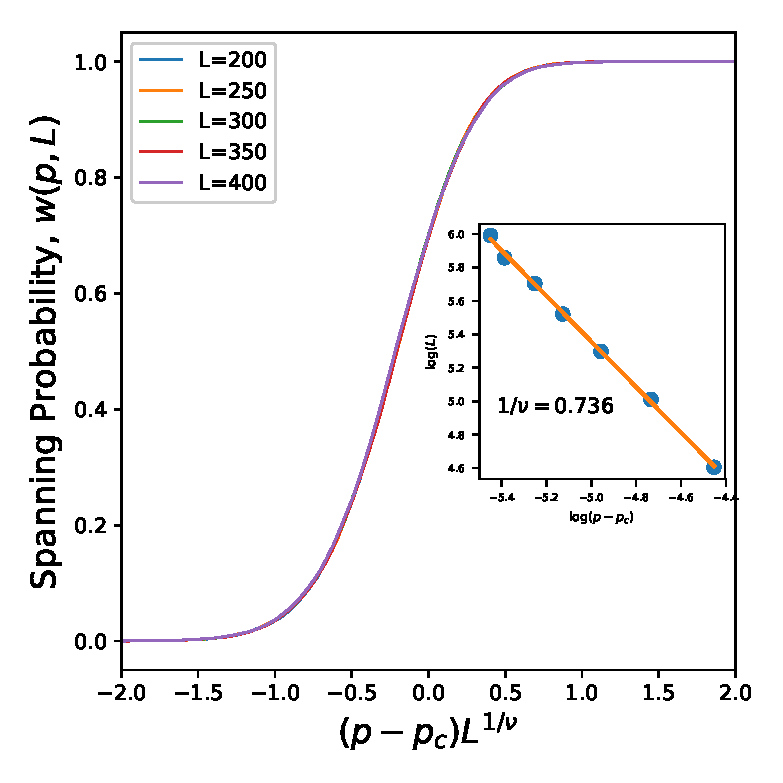
\includegraphics[width=\linewidth]{{{L1/sq_lattice_site_percolation_ballistic_deposition_L1_periodic_-occupation_probability-data_collapse-pc0.5782-ex0.7360}}}
			\caption{}
		\end{subfigure}
		\begin{subfigure}[t]{0.4\textwidth}
			\centering
			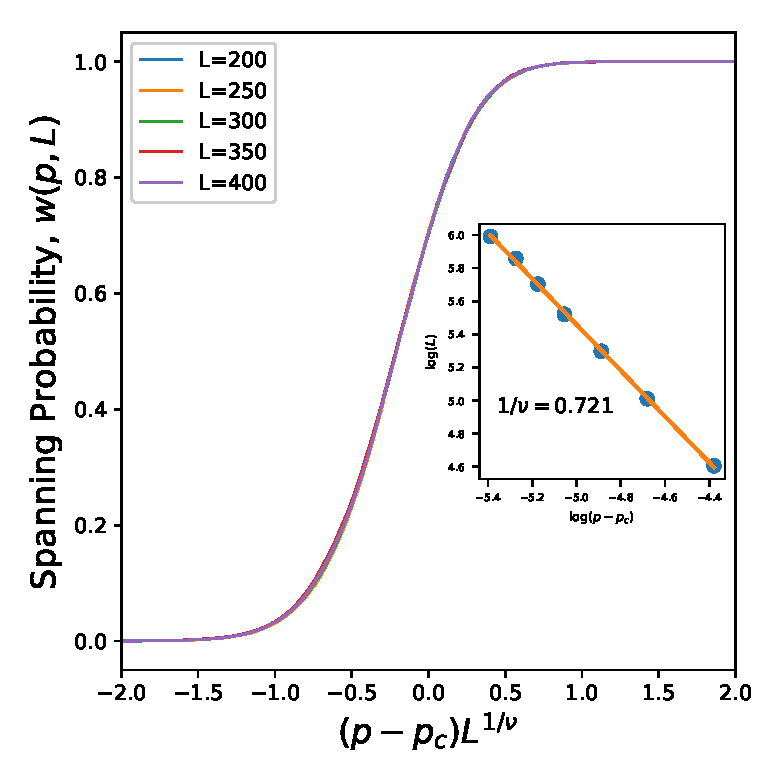
\includegraphics[width=\linewidth]{{{L2/sq_lattice_site_percolation_ballistic_deposition_L2_periodic_-occupation_probability-data_collapse-pc0.5701-ex0.7210}}}
			\caption{}
		\end{subfigure}
		\caption{We plot dimensionless quantities $W$ vs $(p-p_c)L^{1/\nu}$ using value of $1/\nu=0.736,0.721$ respectively for (a) $L1$ and (b) $L2$ for which we find excellent data-collapse. The values of $1/\nu$ is obtained from figure (\ref{fig:spanning-probability-with-hline}) by plotting $\log(L)$ vs $\log(p-p_c)$ which is shown in the inset of this graph.}
		\label{spanning-probability-data-collapse}
	\end{figure}
	

	\subsection{Entropy, Specific Heat and finding $\alpha$}
	\label{subsect:entropy-specific-heat}
		For any phase transition model the entropy is crucial since it determines the type of transition. In percolation theory we use Shannon Entropy \cite{Shannon1948}. Using the definition from section (\ref{subsect:percolation-entropy}) we get the figure (\ref{fig:entropy}).
		\begin{figure}[h]
			\centering
			\captionsetup[subfigure]{width=0.9\textwidth}
			\begin{subfigure}{0.4\textwidth}
				\centering
				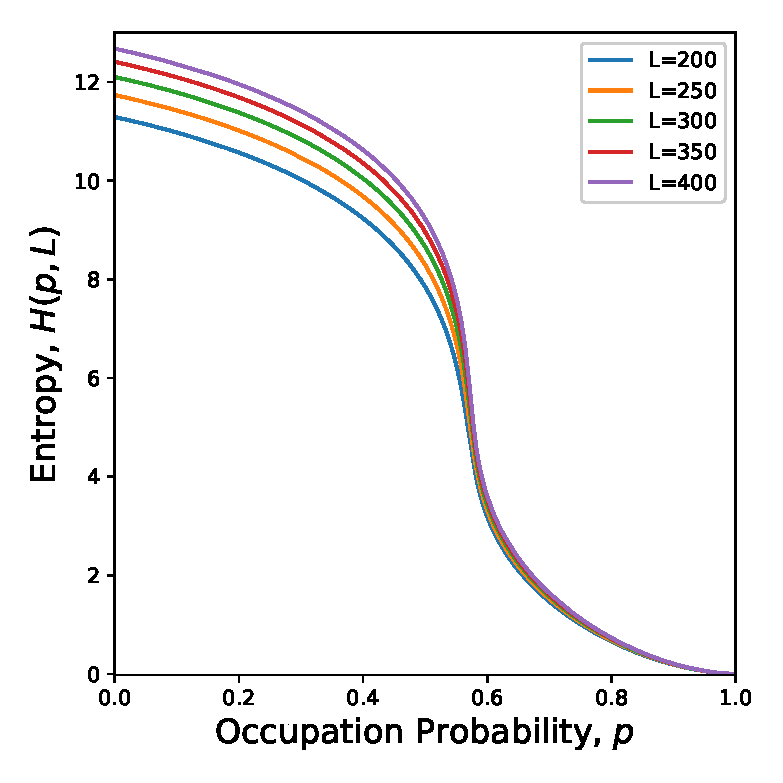
\includegraphics[width=\linewidth]{{{L1/sq_lattice_site_percolation_ballistic_deposition_L1_periodic_-entropy}}}
				\caption{L1}
			\end{subfigure}
			\begin{subfigure}{0.4\textwidth}
				\centering
				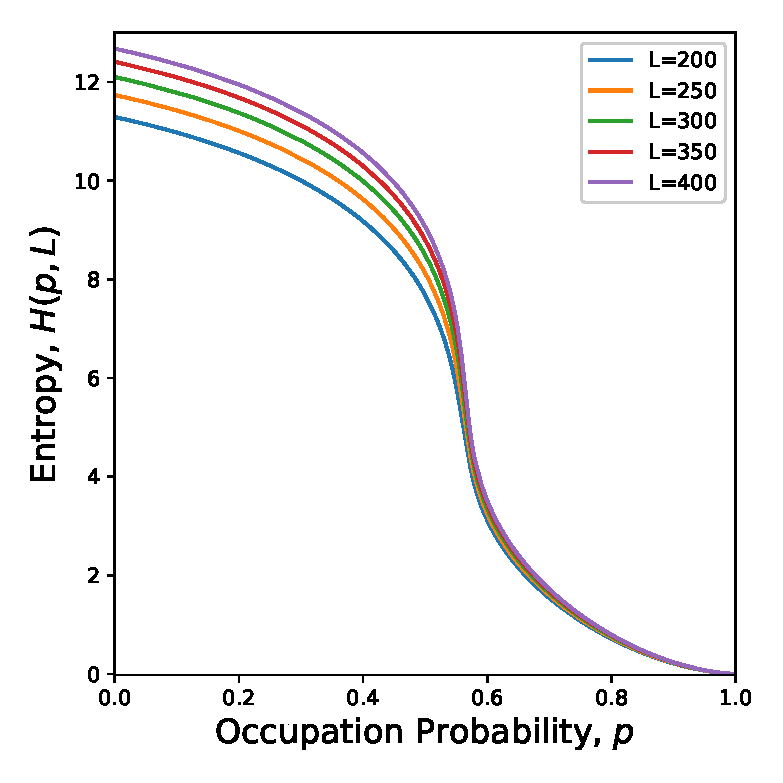
\includegraphics[width=\linewidth]{{{L2/sq_lattice_site_percolation_ballistic_deposition_L2_periodic_-entropy}}}
				\caption{L2}
			\end{subfigure}
			\caption{Entropy, $H(p,L)$ vs Occupation Probability, $p$ for (a) $L1$ and (b) $L2$ interaction in square lattice whose $p_c$ values are $0.5782$ and $0.5701$ respectively}
			\label{fig:entropy}
		\end{figure}
	
	
	Now we attempt to find the specific heat.
		\begin{figure}
		\centering
		\captionsetup[subfigure]{width=0.9\textwidth}
			\begin{subfigure}[t]{0.4\textwidth}
				\centering
				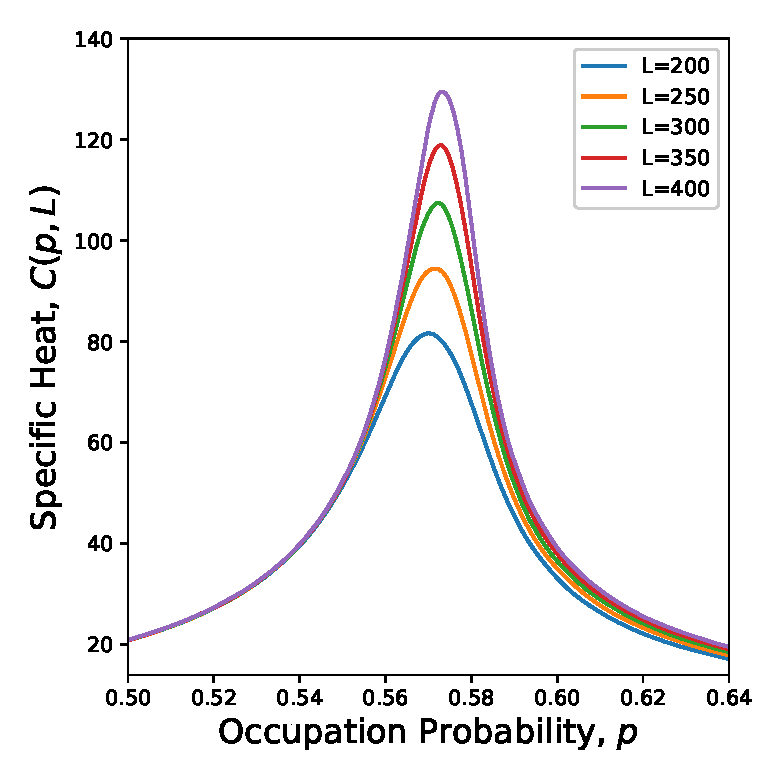
\includegraphics[width=\linewidth]{{{L1/sq_lattice_site_percolation_ballistic_deposition_L1_periodic__specific_heat-pc0.5782}}}
				\caption{}
			\end{subfigure}
			\begin{subfigure}[t]{0.4\textwidth}
				\centering
				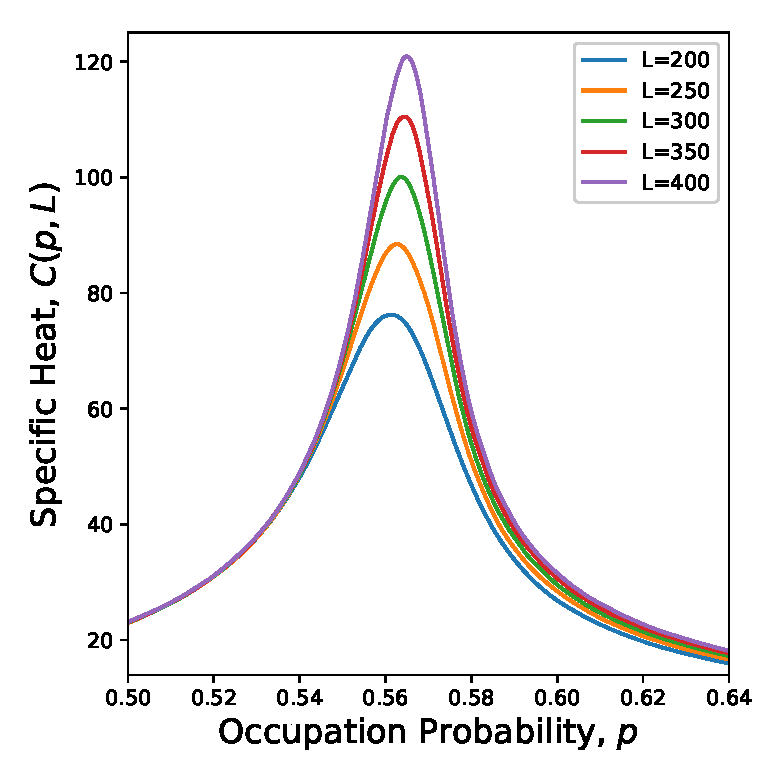
\includegraphics[width=\linewidth]{{{L2/sq_lattice_site_percolation_ballistic_deposition_L2_periodic__specific_heat-pc0.5701}}}
				\caption{}
			\end{subfigure}
			\caption{Specific Heat, $C(p,L)$ vs Occupation Probability, $p$ for (a) $L1$ and (b) $L2$ interaction.}
			\label{fig:specific-heat-graph}
		\end{figure}
	 Since the specific heat $C(p,L)$ is defined in section (\ref{subsect.percolation.specific-heat}), we simply use the relation (\ref{def:specific-heat-percolation}) to obtain the specific heat for percolation in square lattice. But we get a noisy data and we call it micro-canonical. We apply convolution formula to get specific heat for a canonical ensemble. The process of applying convolution is described in appendix (\ref{appendix.convolution}). After applying convolution we a smooth curve shown in figure (\ref{fig:specific-heat-graph}).
	 
		From specific heat we can find the exponent $\alpha$. To do this first we need to scale the $x$-values of the specific heat data using the exponent $1/\nu$ obtained from (\ref{subsect:spanning-probability-and-one-by-nu}) and get the graph as in figure (\ref{fig:specific-heat-x-scaled-graph}).
		\begin{figure}
			\centering
			\captionsetup[subfigure]{width=0.9\textwidth}
			\begin{subfigure}{0.4\textwidth}
				\centering
				\includegraphics[width=\linewidth]{{{sq_lattice_site_percolation_ballistic_deposition_L1_periodic__specific_heat-x-scaled-pc0.5782_alpha_0.6712_nu_0.736}}}
				\caption{}
			\end{subfigure}
			\begin{subfigure}{0.4\textwidth}
				\centering
				\includegraphics[width=\linewidth]{{{sq_lattice_site_percolation_ballistic_deposition_L2_periodic__specific_heat-x-scaled-pc0.5701_alpha_0.6631_nu_0.721}}}
				\caption{}
			\end{subfigure}
			\caption{We plot $C(p,L)$ vs $(p-p_c) L^{1/\nu}$ using values of $1/\nu$ obtained from section (\ref{subsect:spanning-probability-and-one-by-nu}) for (a) $L1$ and (b) $L2$. We then measure height of the curves and call it $C_h$. Then plotting $\log(C_h)$ vs $\log(L)$ gives us the exponent $\alpha/\nu$ which is shown in the inset of figure (\ref{fig:specific-heat-data-collapse-graph})
			}
			\label{fig:specific-heat-x-scaled-graph}
		\end{figure}
	 From this graph we will get the height of each line and call it $C_h$. Since each line corresponds to a specific length $L$ we can plot $\log(C_h)$ versus $\log(L)$ and the absolute value of the graph will give $\alpha/\nu$ and from that we can find the exponent $\alpha$ simply by dividing $\alpha/\nu$ by $1/\nu$. We get $\alpha$ values $0.911,0.919$ for $L1,L2$ correspondingly. and using this value we can apply FSS hypothesis to get data collapse.
	If we plot $C L^{-\alpha/\nu}$ vs $(p-p_c)L^{1/\nu}$ we get perfect data collapse for $L1,L2$ and it is shown in figure (\ref{fig:specific-heat-data-collapse-graph})
	\begin{figure}
		\centering
		\begin{subfigure}{0.4\textwidth}
			\centering
			\includegraphics[width=\linewidth]{{{sq_lattice_site_percolation_ballistic_deposition_L1_periodic__specific_heat-data_collapse-pc0.5782_alpha_0.6712_nu_0.736-with}}}
			\caption{}
		\end{subfigure}
		\begin{subfigure}{0.4\textwidth}
			\centering
			\includegraphics[width=\linewidth]{{{sq_lattice_site_percolation_ballistic_deposition_L2_periodic__specific_heat-data_collapse-pc0.5701_alpha_0.6712_nu_0.721-with}}}
			\caption{}
		\end{subfigure}
		\caption{Plots of dimensionless quantities $C L^{-\alpha/\nu}$ vs $(p-p_c) L^{1/\nu}$ for different sizes of square lattice for (a) $L1$ and (b) $L2$ interaction. We know the values of $1/\nu$ for corresponding interaction from section (\ref{subsect:spanning-probability-and-one-by-nu}). We find excelent data collapse with $\alpha/\nu=0.6712,0.6631$ for (a) $L1$ and (b) $L2$ interaction respectively. Values of $\alpha/\nu$ is obtained from the graph $\log(C_h)$ vs $\log(L)$ which is shown in the inset and $C_h$ is known to us from figure (\ref{fig:specific-heat-x-scaled-graph})}
		\label{fig:specific-heat-data-collapse-graph}
	\end{figure}

	\clearpage
	\newpage
	\subsection{Order Parameter and finding $\beta$}
	\label{subsect:order-parameter}
		Order parameter, also knows as the percolation strength, is ,along with entropy, an important quantity in the study of phase transition. It is denoted as $P(p,L)$. Using the definition (\ref{def:order-parameter}) we obtain the order parameter for our system and it is shown in the figure (\ref{fig:order-parameter}). Since using spanning cluster and the largest cluster gives the same exponent, it really does not matter which one we use. But in our case there is a boundary of the system, which we define as periodic. Hence using spanning cluster is appropriate.
		\begin{figure}[h]
			\centering
			\captionsetup[subfigure]{width=0.9\textwidth}
			\begin{subfigure}{0.4\textwidth}
				\centering
				\includegraphics[width=\linewidth]{{{sq_lattice_site_percolation_ballistic_deposition_L1_periodic_-spanning-_order_parameter-pc0.5782}}}
				\caption{L1}
			\end{subfigure}
			\begin{subfigure}{0.4\textwidth}
				\centering
				\includegraphics[width=\linewidth]{{{sq_lattice_site_percolation_ballistic_deposition_L2_periodic_-spanning-_order_parameter-pc0.5701}}}
				\caption{L2}
			\end{subfigure}
			\caption{Order Parameter, $P(p,L)$ vs Occupation Probability, $p$ for (a) $L1$ and (b) $L2$}
			\label{fig:order-parameter}
		\end{figure}
		Using the exponent $1/\nu$ obtained in section (\ref{subsect:spanning-probability-and-one-by-nu})
		 we scale the $x$-values as $(p-p_c)L^{1/\nu}$ and get the following figure (\ref{fig:order-parameter-x-scaled}).
		\begin{figure}[h]
			\centering
			\begin{subfigure}{0.4\textwidth}
				\centering
				\includegraphics[width=\linewidth]{{{sq_lattice_site_percolation_ballistic_deposition_L1_periodic_-spanning-_order_parameter-x-scaled-pc0.5782}}}
				\caption{}
			\end{subfigure}
			\begin{subfigure}{0.4\textwidth}
				\centering
				\includegraphics[width=\linewidth]{{{sq_lattice_site_percolation_ballistic_deposition_L2_periodic_-spanning-_order_parameter-x-scaled-pc0.5701}}}
				\caption{}
			\end{subfigure}
			\caption{Order Parameter, $P(p,L)$ vs dimensionless quantity $(p-p_c)L^{1/\nu}$ for (a) $L1$ and (b) $L2$ interactions. The values of $1/\nu$ is obtained from section (\ref{subsect:spanning-probability-and-one-by-nu}). We draw a vertical line near the critical point and measure the height of the intersection of the curves of $P$ with the vertical line and call it $P_h$. The plot of $\log(P_h)$ vs $\log(L)$ gives us the exponent $\gamma/\nu$ which is shown in the inset of the figure (\ref{fig:order-parameter-data-collapse})}
			\label{fig:order-parameter-x-scaled}
		\end{figure}
 	    Then in figure (\ref{fig:order-parameter-x-scaled}) we draw a vertical line where there are several horizontal lines. We measure the height of the lines and call it $P_h$ and after plotting $\log(P_h)$ vs $\log(L)$ (inset of figure (\ref{fig:order-parameter-data-collapse}))we get the exponent $\beta/\nu$ from it's slope and obtain exponent $\beta$ by dividing $\beta/\nu$ by $1/\nu$.
 	    Using the FSS hypothesis (\ref{subsect:FSS}) we plot $PL^{\beta/\nu}$ versus $(p-p_c)L^1/\nu$ and get a good data collapse which is shown in figure (\ref{fig:order-parameter-data-collapse}).
		\begin{figure}[h]
			\centering
			\captionsetup[subfigure]{width=0.9\textwidth}
			\begin{subfigure}{0.4\textwidth}
				\centering
				\includegraphics[width=\linewidth]{{{sq_lattice_site_percolation_ballistic_deposition_L1_periodic_-spanning-_order_parameter-data_collapse-pc0.5782_beta_0.103_nu_0.736}}}
				\caption{L1}
			\end{subfigure}
			\begin{subfigure}{0.4\textwidth}
				\centering
				\includegraphics[width=\linewidth]{{{sq_lattice_site_percolation_ballistic_deposition_L2_periodic_-spanning-_order_parameter-data_collapse-pc0.5701_beta_0.098_nu_0.721}}}
				\caption{L2}
			\end{subfigure}
			\caption{We plot $P(p,L)L^{\beta/\nu}$ versus $(p-p_c)L^{1/\nu}$ using the values of $1/\nu$ from section (\ref{subsect:spanning-probability-and-one-by-nu}). And the value of the exponent $\beta/\nu$ obtained from the plot in the inset of this graph. To do this we needed values of $P_h$ which is obtained from figure (\ref{fig:order-parameter-x-scaled}).				An excellent data collapse is obtained using the exponents $\beta/\nu=0.1026,0.0982$ for (a) $L1$ and (b) $L2$ respectively.}
			\label{fig:order-parameter-data-collapse}
		\end{figure}
	
	\clearpage
	\newpage
	\subsection{Susceptibility and finding $\gamma$}
	Susceptibility is defined as the derivative of the order parameter $P(p,L)$ with respect to the control parameter $p$,i.e., $\chi = \frac{dP}{dp}$. Using this definition we obtain the graph of susceptibility (\ref{fig:susceptibility}). 
		\begin{figure}[h]
		\centering
		\captionsetup[subfigure]{width=0.9\textwidth}
			\begin{subfigure}{0.4\textwidth}
				\centering
				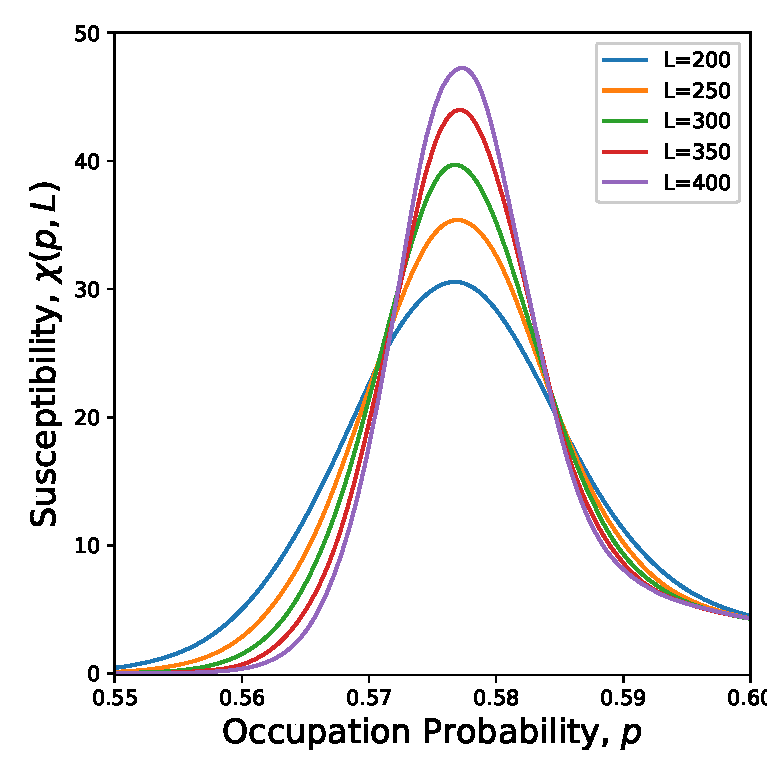
\includegraphics[width=\linewidth]{{{L1/sq_lattice_site_percolation_ballistic_deposition_L1_periodic__susceptibility-pc0.5782}}}
				\caption{L1}
			\end{subfigure}
			\begin{subfigure}{0.4\textwidth}
				\centering
				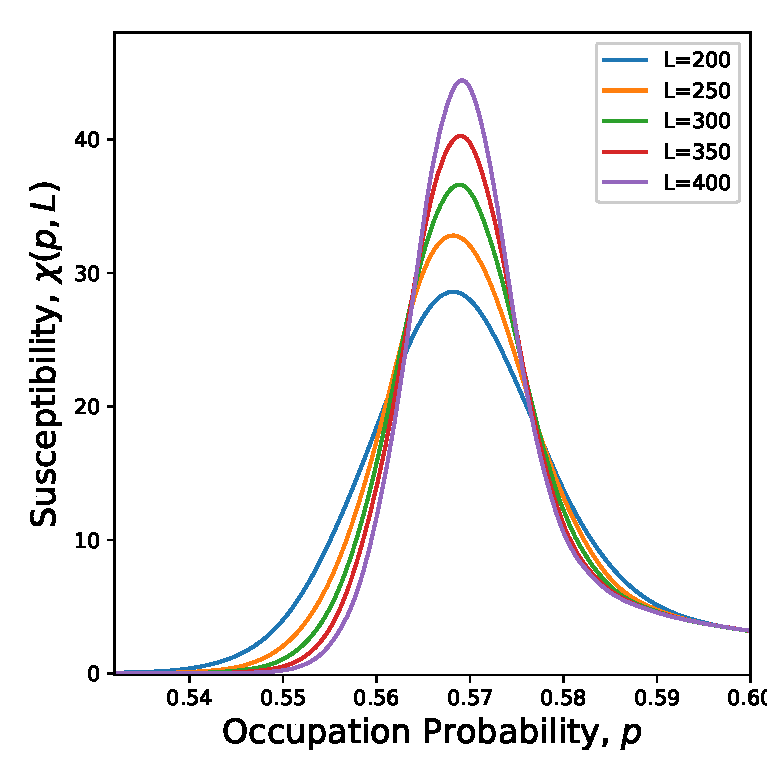
\includegraphics[width=\linewidth]{{{L2/sq_lattice_site_percolation_ballistic_deposition_L2_periodic__susceptibility-pc0.5701}}}
				\caption{L2}
			\end{subfigure}
			\caption{Plots of susceptibility $\chi(p)$ as a	function of $p$ in square lattice of different sizes for (a) $L1$ and (b) $L2$ interaction.}
			\label{fig:susceptibility}
		\end{figure}
	
	And if we scale the $x$ values and plot $\chi$ vs $(p-p_c)L^{1/\nu}$ we get all the peak point aligned (figure (\ref{fig:susceptibility-x-scaled})). Note that the value of $1/\nu$ is known from section (\ref{subsect:spanning-probability-and-one-by-nu}). Then we take the reading of the height of each line and call it $\chi_h$. Since each line represents a different lattice size, plotting $\log(\chi_h)$ vs $\log(L)$ gives the slope $\gamma/\nu$. 
	
		\begin{figure}[h]
			\centering
			\captionsetup[subfigure]{width=0.9\textwidth}
				
			\begin{subfigure}{0.45\textwidth}
				\centering
				\includegraphics[width=\linewidth]{{{sq_lattice_site_percolation_ballistic_deposition_L1_periodic__susceptibility-x-scaled-pc0.5782_gamma_0.6287_nu_0.736}}}
				\caption{}
			\end{subfigure}
			\begin{subfigure}{0.45\textwidth}
				\centering
				\includegraphics[width=\linewidth]{{{sq_lattice_site_percolation_ballistic_deposition_L2_periodic__susceptibility-x-scaled-pc0.5701_gamma_0.6362_nu_0.721}}}
				\caption{}
			\end{subfigure}
			\caption{ We plot $\chi(p,L)$ vs $(p-p_c) L ^{1/\nu}$ using the values of $1/\nu$ obtained from section (\ref{subsect:spanning-probability-and-one-by-nu}). Then we measure the height of the curves and call them $\chi_h$ and plotting $\log(\chi_h)$ vs $\log(L)$ gives us the exponent $\gamma/\nu$ which is shown in the inset of figure (\ref{fig:susceptibility-data-collapse}).}
			\label{fig:susceptibility-x-scaled}
		\end{figure}
	
	And using the FSS hypothesis we plot $\chi L^{-\gamma/\nu}$ vs $(p-p_c)L^{1/\nu}$ and obtain a perfect data collapse. It is shown in figure (\ref{fig:susceptibility-data-collapse}). We obtain the values of $\gamma$ to be $0.8542,0.882$.
	
		\begin{figure}[h]
			\centering
			\captionsetup[subfigure]{width=0.9\textwidth}
			\begin{subfigure}{0.45\textwidth}
				\centering
				\includegraphics[width=\linewidth]{{{sq_lattice_site_percolation_ballistic_deposition_L1_periodic__susceptibility-data_collapse-pc0.5782_gamma_0.6287_nu_0.736}}}
				\caption{}
			\end{subfigure}
			\begin{subfigure}{0.45\textwidth}
				\centering
				\includegraphics[width=\linewidth]{{{sq_lattice_site_percolation_ballistic_deposition_L2_periodic__susceptibility-data_collapse-pc0.5701_gamma_0.6362_nu_0.721}}}
				\caption{}
			\end{subfigure}
			\caption{Plots of dimension less quantities $\chi L^{\gamma/\nu}$ vs $(p-p_c) L ^{1/\nu}$ for different sizes of square lattice for (a) $L1$ and (b) $L2$ interaction. We know the values of $1/\nu$ for corresponding interaction from (\ref{subsect:spanning-probability-and-one-by-nu}). We find excelent data collapse with $\gamma/\nu=0.6287,0.6362$ for (a) $L1$ and (b) $L2$ interaction respectively. Values of $\gamma/\nu$ is obtained from the graph $\log(\chi_h)$ vs $\log(L)$ which is shown in the inset and $\chi_h$ is known to us from figure (\ref{fig:susceptibility-x-scaled})}
			\label{fig:susceptibility-data-collapse}
		\end{figure}
	
	
	\clearpage
	\newpage
	\subsection{Fractal Dimension}
	At critical point the square lattice shows the property of a fractal \cite{Falconer2003} (\ref{subsect:fractal-dim}). We use the relation
	\begin{equation}
	S \sim L^{d_f}
	\label{eqn:fractal-dim}
	\end{equation}
	taking $\log$ we get
	\begin{equation}
	\log(S) = d_f \log(L)
	\end{equation}
	Here $S$ is the average size of the spanning cluster at critical point. Using this we get the figure (\ref{fig:fractal-dimension}). And we obtain fractal dimension $d_f$ for $L0,L1,L2$ which is listed in (\ref{tab:exponents}). 
	\begin{figure}[h]
		\centering
		\captionsetup[subfigure]{width=0.9\textwidth}
		\begin{subfigure}{0.4\textwidth}
			\centering
			\includegraphics[width=\linewidth]{{{sq_lattice_site_percolation_ballistic_deposition_L1_periodic_-fractal_dimension_1.8995}}}
			\caption{}
		\end{subfigure}
		\begin{subfigure}{0.4\textwidth}
			\centering
			\includegraphics[width=\linewidth]{{{sq_lattice_site_percolation_ballistic_deposition_L2_periodic_-fractal_dimension_1.9081}}}
			\caption{}
		\end{subfigure}
		\label{fig:fractal-dimension}
		\caption{We plot $\log(S)$ vs $\log(L)$ where $S$ is the size of the spanning cluster and $L$ is the length of the lattice. We obtain the slope $1.8995$ and $1.9081$ for (a) $L1$ and (b) $L2$ respectively which are the fractal dimensions of the system for $L1$ and $L2$ interactions respectively.}
	\end{figure}
	Fractal dimension gives us the information about the size of the spanning(wrapping) cluster. If the lattice size is known we can estimate the average size of the spanning cluster using $d_f$ and (\ref{eqn:fractal-dim}).
	
	
	\subsection{Order-Disorder Transition}
	Phase transition is an order-disorder transition. There is a critical point which separates the two regions. Before the critical point the system is in disordered phase and after it is in ordered phase when we increase temperature in thermodynamics. Behavior of two phases are completely different. It's astonishing how the behavior changes. In percolation theory, this order disorder transition is different than in thermodynamics.
	
	\begin{figure}
		\centering
		\captionsetup[subfigure]{width=0.9\textwidth}
		\begin{subfigure}{0.4\textwidth}
			\centering
			\includegraphics[width=\linewidth]{{{sq_lattice_site_percolation_ballistic_deposition_L1_periodic_-entropy-order_parameter-L400}}}
			\caption{}
		\end{subfigure}
		\begin{subfigure}{0.4\textwidth}
			\centering
			\includegraphics[width=\linewidth]{{{sq_lattice_site_percolation_ballistic_deposition_L2_periodic_-entropy-order_parameter-L400}}}
			\caption{}
		\end{subfigure}
		\caption{We plot normalized entropy $H(p,L)/H(0,L)$ and normalized order parameter $P(p,L)/P(1,L)$ vs $p$ in one graph to see the order disorder transition in square lattice for (a) $L1$ (b) $L2$ interaction. We had to normalize entropy to make order parameter and entropy comparable.}
		\label{fig:ordered-disordered-transition}
	\end{figure}
	
	 Here disordered means uncertainty, since we are dealing with a system where probability is the control parameter (the occupation probability $p$). When $p$ is minimum all clusters are disconnected and have size of unity. This means that we can to pick a cluster with probability $\frac{1}{2L^2}$, where $L$ is the lattice size and $2L^2$ is the number of bonds in the lattice. That's why entropy is maximum and order parameter is minimum in this region. Now as we keep occupying the lattice clusters of different size arises, and at some point a miracle happens. It is the critical point where the transition occurs. A cluster appears for the first time which spans the entire lattice either horizontally or vertically. And in case of periodic condition the cluster wraps the lattice all the way around it. This cluster is called the spanning (wrapping) cluster in non-periodic (periodic) condition. The probability of picking this cluster at random is always larger than picking any other clusters. Thus system goes to the ordered state. And if we keep occupying the lattice at some point all cluster are joined to form one cluster. Thus picking this cluster at random has no uncertainty, meaning we have reached the entirely ordered phase. Here entropy is minimum and ordered parameter is maximum. A graph (\ref{fig:ordered-disordered-transition}) containing both entropy and order parameter can show this process. We have normalized the entropy (figure (\ref{fig:entropy})) to match with the order parameter (figure (\ref{fig:order-parameter})).
	
	


	
